\documentclass[11pt,a4paper]{article}
\usepackage[margin=2.2cm]{geometry}
\usepackage{booktabs}
\usepackage{graphicx}
\usepackage{amsmath}
\usepackage{float}
\usepackage[hidelinks]{hyperref}

\title{Assignment 8: Multimodal Architecture using Graph Neural Networks}
\author{}
\date{}

\begin{document}
\maketitle
\vspace{-1.5cm}

All experiments use 5,000 products from the Fashion Product Images (Small) dataset, classified into 5 master categories (Apparel, Accessories, Footwear, Free Items, Personal Care). Image embeddings (64-d) are extracted from a pretrained ResNet18 and text embeddings (64-d) via SVD-projected bag-of-words on product names. The data is split 80/20 for training and testing.

\section{Part A: GNN on Bipartite Graphs}

We construct a bipartite graph with two node types: image nodes and text nodes (5,000 each, 10,000 total). Three edge types connect them: Image-Image and Text-Text edges via $k$-NN ($k{=}5$) on cosine similarity (25,000 edges each), and Image-Text edges linking each product's image and text nodes bidirectionally (10,000 edges). A single message passing layer aggregates neighbour features ($\mathbf{m}_i = \sum_{j} W_\text{msg}\mathbf{h}_j$, update: $\mathbf{h}_i' = \text{ReLU}(W_\text{upd}[\mathbf{h}_i \| \mathbf{m}_i])$). Product-level predictions are obtained by averaging each product's image and text node representations.

\begin{figure}[H]
\centering
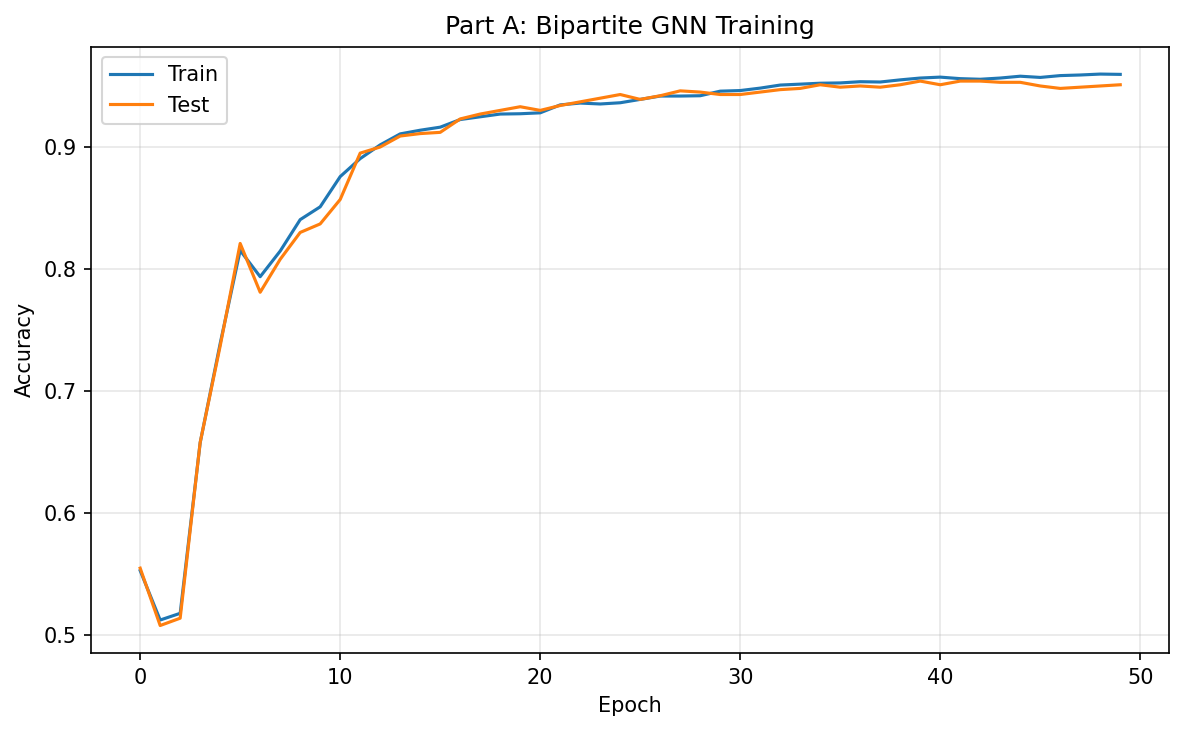
\includegraphics[width=0.65\textwidth]{part_a_training.png}
\caption{Part A: Bipartite GNN training and test accuracy.}
\end{figure}

The bipartite GNN reaches 95.4\% test accuracy. The cross-modal edges are crucial: they allow image features to inform text representations and vice versa during message passing, creating richer multimodal node embeddings than either modality alone.

\section{Part B: Fusion Strategies}

We compare the bipartite GNN against two fusion approaches and implement cross-modal retrieval.

\textbf{Early fusion} concatenates image and text embeddings into a 128-d vector, projects through an MLP to 64-d, then runs one message passing layer on a $k$-NN graph built from the fused features. \textbf{Late fusion} runs two independent GNNs on separate image and text similarity graphs, then concatenates their outputs and classifies via an MLP.

\begin{table}[H]
\centering
\begin{tabular}{lc}
\toprule
Model & Best Test Acc \\
\midrule
Bipartite GNN (Part A) & 0.954 \\
Early Fusion GNN & \textbf{0.981} \\
Late Fusion GNN & 0.977 \\
\bottomrule
\end{tabular}
\caption{Fusion strategy comparison.}
\end{table}

Early fusion outperforms both alternatives because fusing features before graph construction creates a unified similarity space where neighbours are truly multimodally similar, leading to more informative message passing. Late fusion performs well but lacks cross-modal interaction during message passing -- each GNN only sees its own modality. The bipartite GNN falls between, as cross-modal edges exist but the graph is more complex to optimise.

\textbf{Cross-modal retrieval} uses the early fusion GNN: a query from one modality (with zeros for the other) is projected through the model's fusion layer and compared via cosine similarity against all GNN-learned embeddings. Retrieval accuracy is low because zeroing out an entire modality creates an out-of-distribution input that the fusion MLP was not trained to handle -- a known limitation of simple concatenation-based fusion.

\begin{figure}[H]
\centering
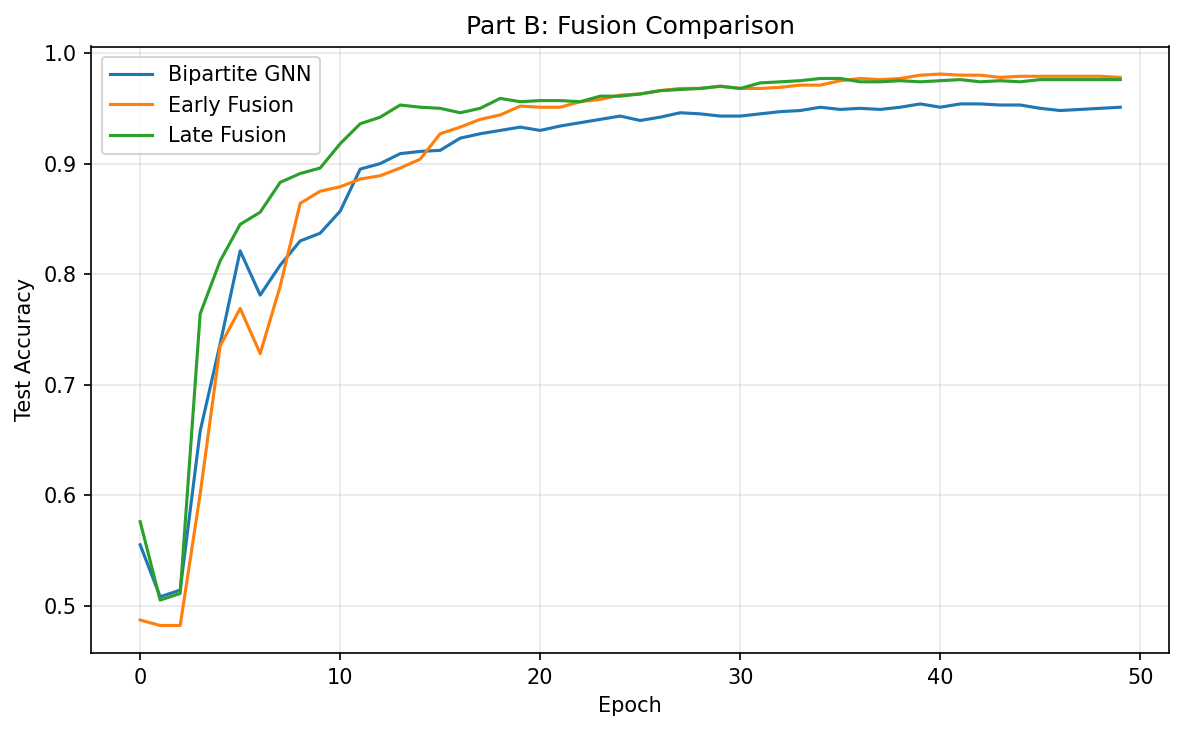
\includegraphics[width=0.7\textwidth]{part_b_fusion.png}
\caption{Test accuracy comparison across fusion strategies.}
\end{figure}

\section{Part C: Semi-supervised Learning}

We train with limited labels (5\%, 10\%, 20\%) using four strategies: supervised-only cross-entropy, pseudo-labelling (high-confidence predictions used as labels every 5 epochs), Mean-Teacher (EMA teacher with consistency regularisation), and both combined.

\begin{table}[H]
\centering
\begin{tabular}{lccc}
\toprule
Method & 5\% & 10\% & 20\% \\
\midrule
Supervised only & 0.933 & 0.942 & 0.955 \\
+ Pseudo-labels & 0.925 & 0.944 & 0.955 \\
+ Mean-Teacher & 0.932 & \textbf{0.953} & 0.953 \\
+ Both & \textbf{0.936} & 0.947 & \textbf{0.958} \\
\bottomrule
\end{tabular}
\caption{Semi-supervised learning across label fractions.}
\end{table}

\begin{figure}[H]
\centering
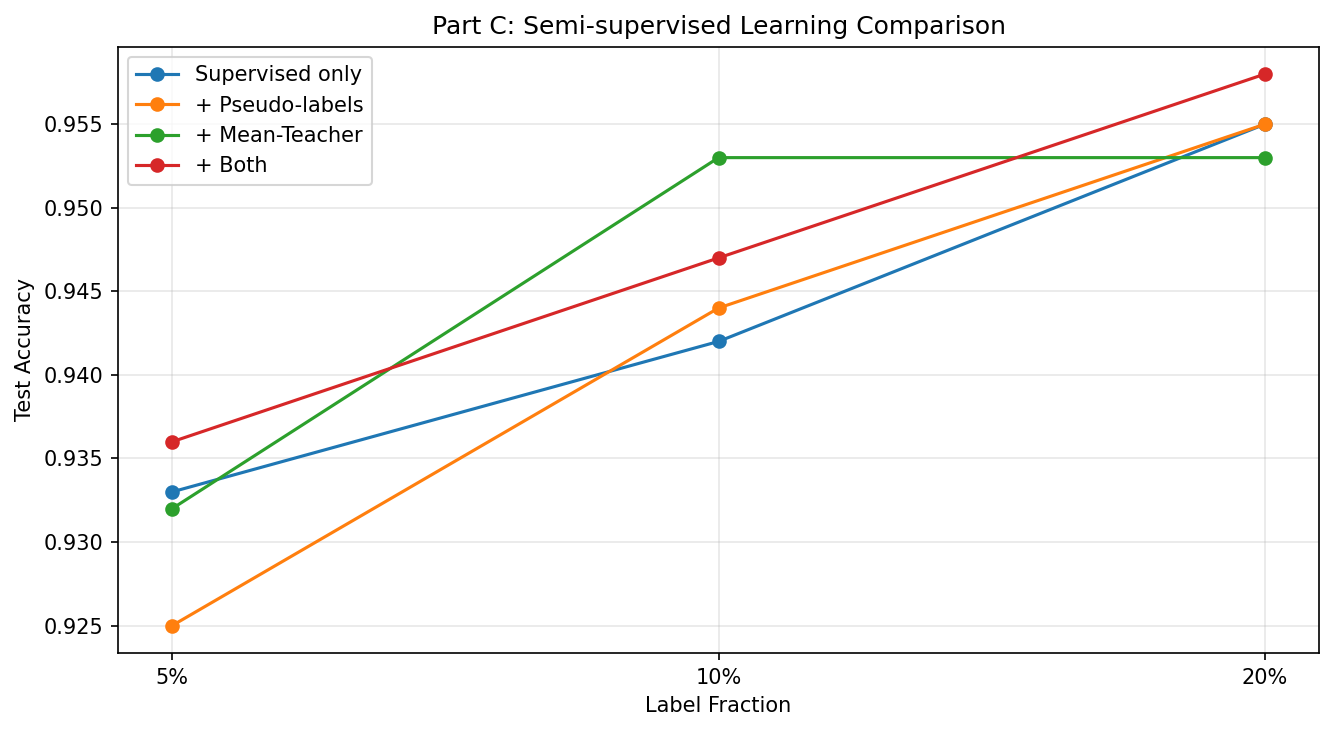
\includegraphics[width=0.7\textwidth]{part_c_semisupervised.png}
\caption{Test accuracy vs label fraction for each semi-supervised method.}
\end{figure}

The combined approach (pseudo-labels + Mean-Teacher) performs best overall, gaining 0.3--0.5 points over supervised-only at low label fractions. Mean-Teacher is particularly effective at 10\% labels (+1.1 points) because consistency regularisation leverages the GNN's graph structure to propagate information from labelled to unlabelled nodes through their shared neighbourhood. Pseudo-labels alone can hurt at very low label fractions (5\%) because early pseudo-labels are unreliable and introduce noise.

\section{Part D: Self-supervised Contrastive Learning}

We pretrain a GNN encoder using InfoNCE contrastive loss on two augmented graph views created by edge dropout (20\%), feature masking (20\%), and feature jitter ($\sigma{=}0.05$). After 100 pretraining epochs, we freeze the encoder and evaluate with a linear probe and $k$-NN.

\begin{table}[H]
\centering
\begin{tabular}{lc}
\toprule
Evaluation & Accuracy \\
\midrule
Linear probe (frozen) & 0.721 \\
$k$-NN ($k{=}3$) & 0.911 \\
$k$-NN ($k{=}5$) & 0.912 \\
$k$-NN ($k{=}10$) & 0.885 \\
\bottomrule
\end{tabular}
\caption{Contrastive embedding quality evaluation.}
\end{table}

\begin{figure}[H]
\centering
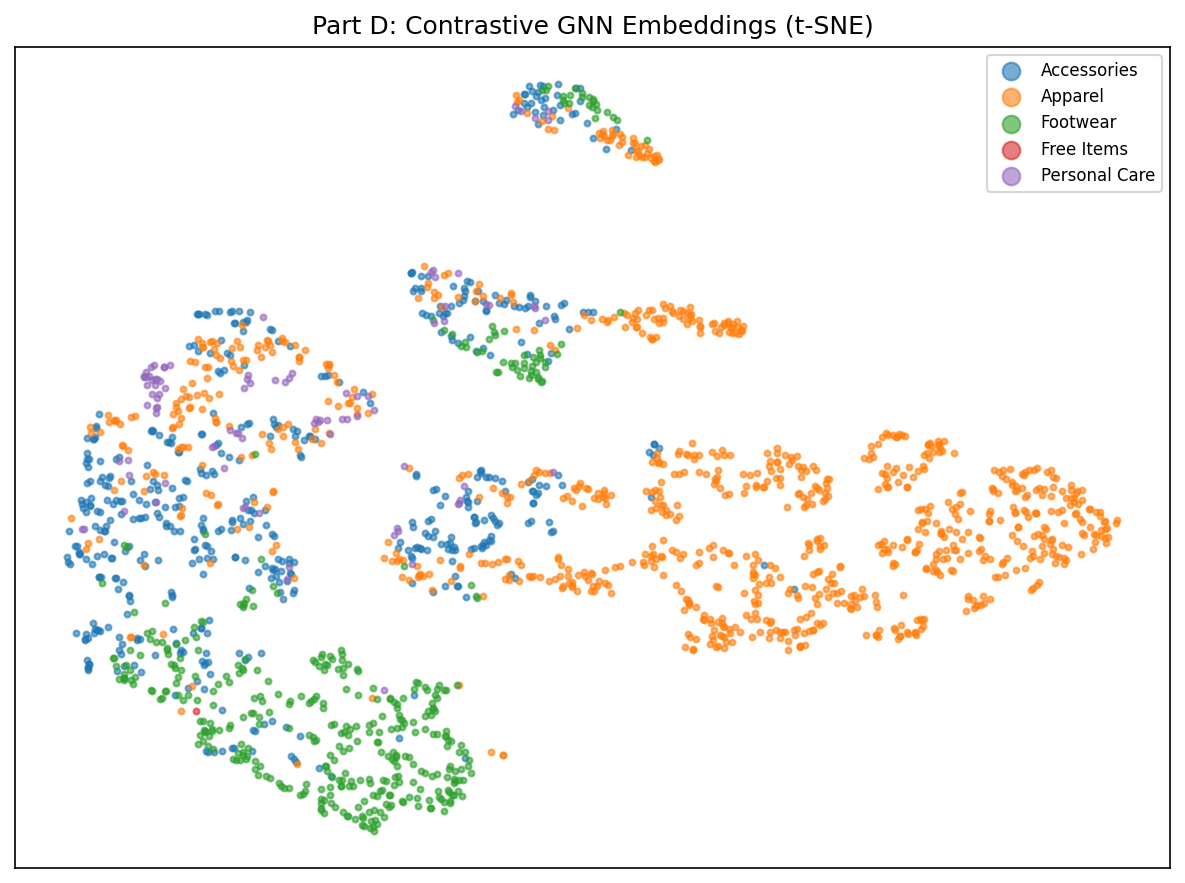
\includegraphics[width=0.7\textwidth]{part_d_tsne.png}
\caption{t-SNE of contrastive GNN embeddings coloured by category.}
\end{figure}

The $k$-NN accuracy (91.2\%) significantly exceeds the linear probe (72.1\%), indicating the learned embeddings form well-separated clusters in a non-linearly structured space. The t-SNE visualisation confirms clear category clusters with Footwear and Apparel well-separated. The gap to supervised accuracy (95--98\%) is expected since contrastive pretraining uses no labels. These embeddings could serve as strong initialisations for downstream fine-tuning with limited labels, complementing the semi-supervised approaches from Part~C.

\end{document}
